\documentclass[10pt,twocolumn,letterpaper]{article}

\usepackage{enumitem}
\usepackage{cvpr}
\usepackage{times}
\usepackage{epsfig}
\usepackage{graphicx, color, xcolor}
\usepackage{amsmath}
\usepackage{amssymb}
\usepackage{bm}
\usepackage[utf8]{inputenc}
\usepackage{fancyhdr}
\usepackage[brazil, english]{babel}
\setlength{\headheight}{1.5cm}
\usepackage{threeparttable}
\usepackage{float}
\usepackage{placeins}
\usepackage{amsmath}
\usepackage{tikz}
\usepackage{pgfplots}
\usetikzlibrary{patterns}
\usepackage{circuitikz}
\usepackage{caption}
\captionsetup[table]{name=Table}
\renewcommand{\thetable}{\arabic{table}}
\usepackage{siunitx}
\usepackage{booktabs}
\usepackage{array}
\usepackage{xcolor}
\usepackage{graphicx}
\usepackage{listings}
\setlist[itemize]{itemsep=0.3em, parsep=0pt, topsep=0.5em}

\fancypagestyle{plain}{%\fancyhf{}%}
\lhead{
\includegraphics[width=5cm]{image/unb.pdf}}
\rhead{
\includegraphics[width=5.9cm]{image/dep.pdf}}

\renewcommand{\headrulewidth}{1pt}%
}

% Changing the caption and 'References' names to Portuguese.
\addto\captionsenglish{
  \renewcommand{\abstract}{Resumo} % Traduzindo o abstract inicial
  \renewcommand{\figurename}{Figura}
  \renewcommand{\tablename}{Tabela}
  \renewcommand{\refname}{Referências bibliográficas}
}
\renewcommand{\lstlistingname}{Código}
\renewcommand{\lstlistlistingname}{Código}
\renewcommand{\abstractname}{Resumo}


% to-do: Using fontenc with T1 font encoding allows \hyphenation to take words with accents
% as arguments. However, fontenc with T1 mess up with words containing 'ã' in all \subsection{}
% commands.
% If someone knows how to fix it, tell me!
%
%\usepackage[T1]{fontenc}

% Put the words not correctly hyphenated down here. Words with accents must
% be manually hyphenated in the text itself using the '\-' separator. See the examples
% throughout this template.
\hyphenation{co-e-ren-te u-sa-do de-li-mi-ta-do-res a-cer-ca va-lo-res cor-res-pon-den-te re-fe-ren-ci-a-das co-lu-na co-lu-nas em-bo-ra u-ti-li-da-de pro-ce-di-men-to ex-pe-ri-men-to fi-gu-ras}

% If you comment hyperref and then uncomment it, you should delete
% egpaper.aux before re-running latex.  (Or just hit 'q' on the first latex
% run, let it finish, and you should be clear).
\usepackage[breaklinks=true,bookmarks=true]{hyperref}

\cvprfinalcopy % *** Uncomment this line for the final submission

\begin{document}
\title{5º experimento - Dispositivos semicondutores fotoemissores e fotoreceptores}

\author{Larissa Simões\\
{\tt\small 232028230@aluno.unb.br}\\
{\tt\small 23/2028230}\\
{\tt\small Turma 1A}
\and
Carlos Eduardo da S. Papa\\
{\tt\small 232013390@aluno.unb.br}\\
{\tt\small 23/2013390}\\
{\tt\small Turma 1A}
\and
Thiago Ferreira\\
{\tt\small 232028230@aluno.unb.br}\\
{\tt\small 23/2028230}\\
{\tt\small Turma 1A}
}

\maketitle

\begin{abstract}
Este experimento estuda dispositivos semicondutores fotoemissores e fotoreceptores, baseando-se na interação entre fótons e portadores de carga1. Os procedimentos incluem o levantamento da curva $I_D \times V_D$ de um LED e da curva $I_C \times V_{CE}$ de um fototransistor sob variadas condições de iluminação2. Serão também analisadas as tensões e correntes em fotocélulas3. Por fim, implementa-se um sistema de acoplamento óptico para avaliar a fidelidade na transmissão de sinais e o comportamento dinâmico do conjunto emissor-receptor.
\end{abstract}

%%%%%%%%%%%% OBJETIVOS %%%%%%%%%%%%%
\section{OBJETIVOS}

\noindent\hspace{.3cm}Determinar, a partir do gráfico $I_D \times V_D$ de um diodo, a tensão de limiar a partir da qual a emissão de luz se torna perceptível. Verificar a dependência da resistência de um fototransistor em relação à potência luminosa incidente em uma faixa de frequência específica. Analisar o funcionamento e as curvas características de células solares, bem como o comportamento de sistemas de acoplamento óptico.

\vspace{.25cm}



 %%%%%%%%%%%
%%%%%%%%%%%%%%%%%%%%%%%%%%%%%%%%%%%%

%%%%%%%%%%%% MATERIAIS %%%%%%%%%%%%%
\section{MATERIAIS E EQUIPAMENTOS UTILIZADOS}

\begin{itemize}
    \item Multímetros digitais;
    \item Diodo emissor de luz;
    \item Resistores $(100 \,\Omega $ e $1k \,\Omega )$;
    \item Fototransistor TIL78;
    \item Cabos para conexões;
    \item Células fotoelétricas;
    \item Lâmpada;
    \item Caixa cilíndrica metalizada;
    \item Circuito de um acomplamento óptico;
    \item Osciloscópio Agilent;
    \item Fonte LEEPUC Mod.402-A;
    \item Fonte de tensão Varivolt;
\end{itemize}

\vspace{.25cm} %%%%%%%%%%%
%%%%%%%%%%%%%%%%%%%%%%%%%%%%%%%%%%%%

%%%%%%%%%%%% PROCEDIMENTOS %%%%%%%%%%%%
\section{PROCEDIMENTOS}

\emph{A. Fotodiodo}

Realiza-se a montagem do circuito abaixo e levanta-se a curva característica IDxVD, variando-se a tensão na fonte de 0 V a 5 V em passos de 200 mV.

% Imagem Circ 1 - font -> resistência -> led

\emph{B. Fototransistor}

Monta-se o circuito abaixo cuja a resistência é controlável pela potência luminosa incidente sobre ele numa dada faixa do espectro de frequências. Em seguida, levanta-se a característica ICxVce do fototransistor TIL78 nas seguintes condições: Sob luz incidente, com iluminação extra de uma lâmpada controlada por um varivolt em 60 mV, mesma iluminação extra porém com o varivolt em 80 mV. Para levantar a curva nas condições citadas acima, deve-se variar a tensão na fonte de 0 a 6 V em passos de 0,5 V, determinando a corrente no dispositivo e a tensão entre seus terminais em cada caso.

% Imagem Circ 2 - font -> resistência -> fotoresistor 

\emph{C. Fotocélulas}

Com o uso de fotocélulas, mede-se a tensão de circuito aberto e a corrente de curto-circuito em diferentes condições de iluminação incidente na fotocélula.

\emph{D. Acoplamento óptico}

Monta-se o circuito abaixo de acoplamento óptico e, colocando-se uma tensão V1 na fonte, verifica-se o comportamento captado pelo fototransistor através do osciloscópio.

% Imagem Circ 3 - acoplamento óptico (transmissão de sinais entre sistemas eletrônicos por meio de luz)

\vspace{.25cm} %%%%%%%%%%
%%%%%%%%%%%%%%%%%%%%%%%%%%%%%%%%%%%%%%%

%%%%%%%%%%% RESULTADOS E ANÁLISE DOS RESULTADOS %%%%%%%%%%%
\section{RESULTADOS EXPERIMENTAIS}

\subsubsection*{A. Fotodiodo}

Seguindo os passos do procedimento foi construida a Tabela \ref{tab:circ1}:

\input{r5-resultados-Table1.tex}

\subsubsection*{B. Fototransistor}

Seguindo o procedimento do item "b" do roteiro foram recolhidos os dados que constam na Tabela \ref{tab:circ2}.

% Tabela 2 - Varivolt = 60 mV e Varivolt = 80 mV
\begin{table}[!h]
    \centering
    \caption{Tensão e corrente do Fototransistor}
    \label{tab:circ2}
    \vspace{0.25cm}
    \begin{tabular}{c|cc|cc} 
        \hline
        \rule{0pt}{3ex} & \multicolumn{2}{c}{\textbf{60} [V]} & \multicolumn{2}{c}{\textbf{80} [V]} \\
        \cline{2-5} 
        \rule{0pt}{3ex}\textbf{V}$_{fonte}$ [V] & $\mathbf{V}_{D}$ [V] & $\mathbf{I}_{D}$ [A] & $\mathbf{V}_{D}$ [V] & $\mathbf{I}_{D}$ [A] \\[5pt]
        \hline
        \rule{0pt}{3ex}0.0 & 0.0 & 0.0 & 0.0 & 0.0 \\
        0.5 & 0.17 & 0.33 & 0.11 & 0.4 \\
        1.0 & 0.48 & 0.52 & 0.15 & 0.89 \\
        1.5 & 0.97 & 0.54 & 0.18 & 1.36 \\
        2.0 & 0.87 & 1.18 & 0.22 & 1.86 \\
        2.5 & 1.5 & 1.04 & 0.34 & 2.25 \\
        3.0 & 1.8 & 1.24 & 0.57 & 2.52 \\
        3.5 & 2.44 & 1.12 & 1.16 & 2.44 \\
        4.0 & 2.87 & 1.18 & 1.44 & 2.69 \\
        4.5 & 3.26 & 1.29 & 1.97 & 2.64 \\
        5.0 & 3.81 & 1.25 & 2.55 & 2.56 \\
        5.5 & 4.21 & 1.36 & 3.48 & 2.16 \\
        6.0 & 4.8 & 1.27 & 3.53 & 2.58 \\ [5pt]
        \hline
    \end{tabular}
\end{table}


\subsubsection*{C. Fotocélulas}

Para este procedimento, a professora realizou a prévia montagem do circuito conforme especificações do roteiro e foram recolhidos os dados que compoem a Tabela \ref{tab:circ3}.

% Tabela 4 - TEnsão de Circuito aberto e corrente de curto circuito da Fotocélula
\begin{table}[!h]
    \centering
    \caption{Tensão e corrente das Fotocélulas}
    \label{tab:circ3}
    \vspace{0.25cm}
    \begin{tabular}{ccc}
        \hline
        \rule{0pt}{3ex}\textbf{Entrada} & \textbf{\textbf{V}}$_{out}$ [V] & \textbf{\textbf{I}}$_{out}$ [A] \\[5pt]
        \hline
        \rule{0pt}{3ex}Escuro & 0.01 & 0 \\
        Claro & 0.41 & 0.01 \\
        60.0 V & 1.9 & 21.8 \\
        80.0 V & 2 & 46.7 \\
        100.0 V & 2.11 & 100.4 \\
        120.0 V & 2.18 & 163.0 \\
        140.0 V & 2.24 & 260 \\
        160.0 V & 2.26 & 350 \\
        180.0 V & 2.27 & 490 \\ [5pt]
        \hline
    \end{tabular}
\end{table}


\subsubsection*{D. Acoplamento óptico}

Novamente com a abordagem de experimento desmonstrativo, a professora construiu um sistema rudimentar de acoplamento óptico e que foi registratado através das figuras \ref{fig:fotos1}, \ref{fig:fotos2} e \ref{fig:fotos3}.

% Foto 1 do ociloscópio
\begin{figure}[h]
\centering
\fbox{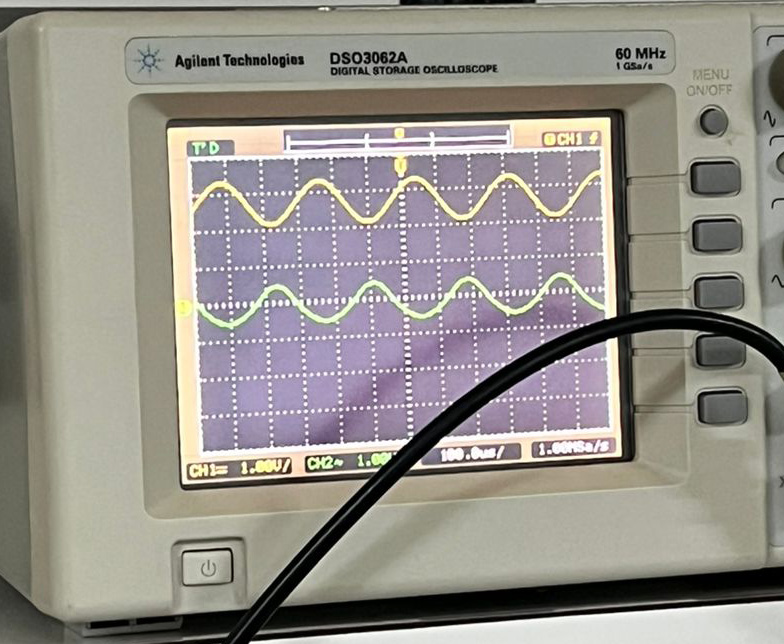
\includegraphics[width=5cm]{fotos/1.jpeg}}
\caption{Modulação e Polarização}
\label{fig:fotos1}
\end{figure}

% Foto 2 do ociloscópio
\begin{figure}[h]
\centering
\fbox{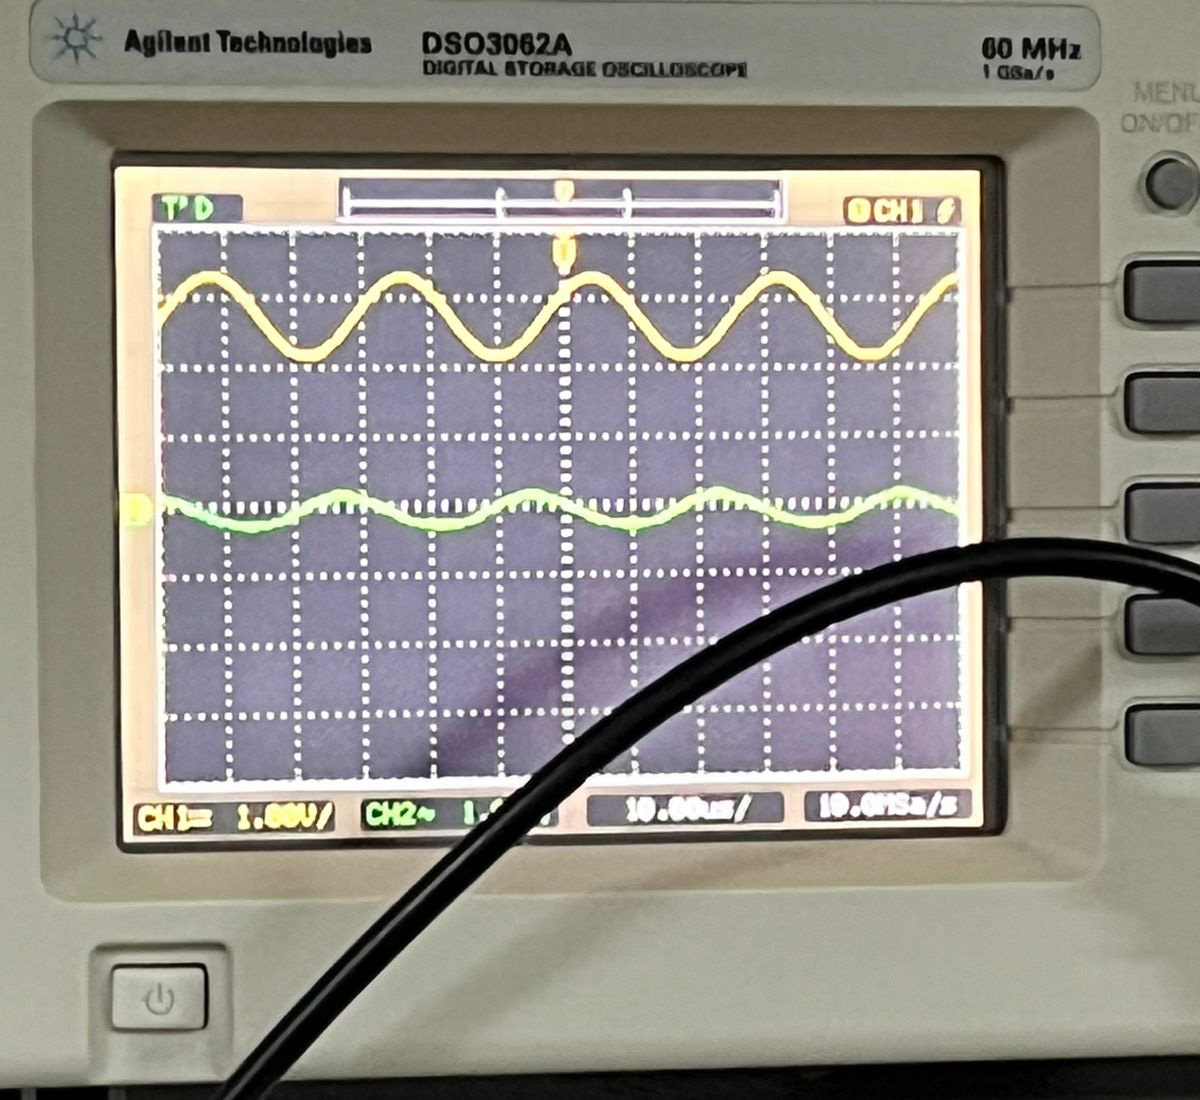
\includegraphics[width=5cm]{fotos/2.jpeg}}
\caption{Defasagem e Inversão de Fase}
\label{fig:fotos2}
\end{figure}

% Foto 3 do ociloscópio
\begin{figure}[h]
\centering
\fbox{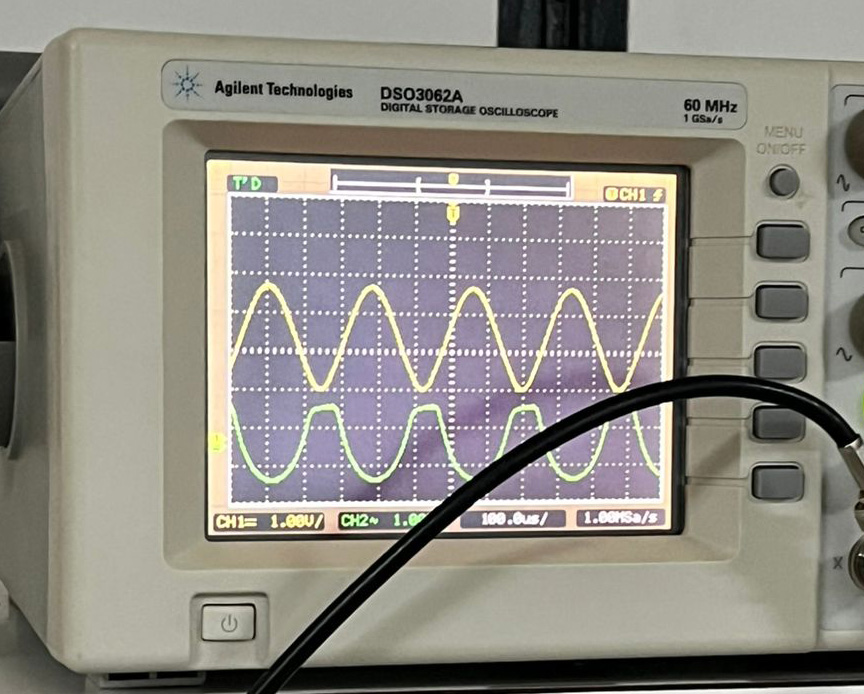
\includegraphics[width=5cm]{fotos/3.jpeg}}
\caption{Saturação e Corte}
\label{fig:fotos3}
\end{figure}

\vspace{.25cm}  %%%%%%%%%%%%%%%%%%%%%%%%%%%%%%%%
%%%%%%%%%%%%%%%%%%%%%%%%%%%%%%%%%%%%%%%%%%%%%%%%%%%%%%%%%%%

%%%%%%%%%%%% CONCLUSÕES %%%%%%%%%%%%%%
\section{CONCLUSÕES}

Nesse experimento pudemos verificar o princípio de funcionamento do LED, do fototransistor e da fotocélula. Com os circuitos montados aplicamos sinais de entrada (tensão) com valores distintos e assim montamos as curvas características do LED, do fototransistor e da fotocélula podendo assim ver o comportamento exponencial de suas curvas. Por fim a partir de um circuito com acoplamento óptico foi possível entender as limitações do LED e do fototransistor fazendo uma comparação entre os sinais antes e depois da mudança tanto da amplitude de entrada quanto da frequéncia. %%%%%%%%%%%%
%%%%%%%%%%%%%%%%%%%%%%%%%%%%%%%%%%%%%%

%%%%%%%%%%%%% REFERÊNCIAS BIBLIOGRÁFICAS %%%%%%%%%%%%%%%%%%%%%%%%%
{\small \bibliography{egbib} \bibliographystyle{ieee_fullname}} %%%
%%%%%%%%%%%%%%%%%%%%%%%%%%%%%%%%%%%%%%%%%%%%%%%%%%%%%%%%%%%%%%%%%%

%%%%%% APENDICES %%%%%%%%
% \appendix %%%%%%%%%%%%%%%
%%%%%%%%%%%%%%%%%%%%%%%%%

%%%%% SCRIPT PYTHON %%%%%%%%%%%%%%%%
% \input{r5-apendice-script.tex} %%%%%
%%%%%%%%%%%%%%%%%%%%%%%%%%%%%%%%%%%%

\end{document}